%\documentclass[11pt,a4paper]{book}
\documentclass[10pt,b5paper,twoside]{book}

% Line spacing
%\linespread{1.0}

% Include document setup script
% Document properties
\usepackage[twoside,paperwidth=176mm,paperheight=250mm,left=2.5cm,right=2cm,top=3cm,bottom=3.0cm]{geometry} % Margins as described by Tapir
\usepackage[comma,sort&compress,square]{natbib}
\usepackage{bibunits}
\usepackage{amsfonts}
\usepackage{amsmath}
\usepackage{fancyhdr}
\usepackage[breaklinks=true,bookmarks=true,citecolor=blue,bookmarksopen=false,bookmarksnumbered=false,bookmarkstype=toc,colorlinks=true,linkcolor=blue,linktocpage]{hyperref}
\hypersetup{ pdfauthor = {Jon Petter \AA{}sen},
             pdftitle = {},
             pdfsubject = {},
             pdfkeywords = {Real-Time Capon Beamforming, Minimum Variance Beamforming, Graphics Processing Unit, GPGPU, Adaptive Visualization, }}

%\usepackage{cite}      % Written by Donald Arseneau
\usepackage[latin1]{inputenc} %To get the norwegian ��� printed correct.
\usepackage{graphicx}  % Written by David Carlisle and Sebastian Rahtz
\usepackage[tight,normalsize]{subfigure} % Written by Steven Douglas Cochran
\usepackage{url}       % Written by Donald Arseneau
\usepackage{bm} % bold math
\usepackage{tabularx}
\usepackage{placeins} % Keep figures within sections

% Settings
% Matrix and vector notation
\newcommand{\matdef}{\mathbf} % Defined finite matrix
\newcommand{\matndef}{\mathbf} % Undefined matrix
\newcommand{\vectdef}{\mathbf} % Defined finite vector
\newcommand{\vectndef}{\bm} % Undefined vector
\newcommand{\change}{\textrm}
\newcommand{\changeSecRev}{\textrm}

% Define department command
\newcommand{\department}[1]{\def\thedepartment{#1}}
\department{(department ikke spesifisert)}

\renewcommand{\contentsname}{Table of Contents}  % Original name = Contents
\renewcommand{\bibname}{References}  % Original name = Bibliography
\newcommand{\runningtitle}[1]{\chaptermark{#1}}
\newcommand{\runningtitleTwo}[1]{\sectionmark{#1}}
\newcommand{\initial}{\relax}
\newcommand{\authors}[2]{\vspace*{-1cm}{\large #1}\\#2\par\vspace{\baselineskip}}
\newcommand{\authorsSmall}[2]{\vspace*{-0.15cm}{\small #1}\\ {\small #2}\par\vspace{\baselineskip}}

\hyphenpenalty=8000 \tolerance=2000
\renewcommand{\topfraction}{0.85}
\renewcommand{\textfraction}{0.1}
\renewcommand{\floatpagefraction}{0.75}

% Headers and footers
\pagestyle{fancy} \fancyhf{} \fancyhead[LO]{\nouppercase{\leftmark}}
\fancyhead[RE]{\nouppercase{\rightmark}}
\cfoot{\rm\thepage} % page number

% Renew maketitle for custom title page
\makeatletter
\renewcommand{\maketitle}{%
\thispagestyle{empty}
\begin{minipage}{14cm}
\raggedright
{\ }\\
{\LARGE\@author}
{\ }\\{\ }\\{\ }\\
{\huge\@title}\\
\vspace*{0.3\textheight}
{\ }\\
%{\ }\\
{\large Thesis for the degree of Philosophiae Doctor}
{\ }\\{\ }\\
\large Trondheim, 1. March 2014\\
{\ }\\
{\large Norwegian University of Science and Technology\\
Faculty of Medicine\\
\thedepartment\\\vspace{1.9cm}

\includegraphics[width=6cm]{./images/NTNULogoEng.pdf}
}
\end{minipage}

\let\maketitle\relax
} \makeatother

% Define abstract enviroment
\newenvironment{abstract}{\begin{minipage}[c]{0.9\columnwidth}\initial}{\end{minipage}}

% Define preface enviroment
\makeatletter
\newenvironment{preface}{\chapter*{Preface}%
\thispagestyle{empty}
\begin{minipage}{0.9\textwidth}
This thesis is submitted in partial fulfilment of the requirements
for the degree of PhD at the Norwegian University of Science and
Technology (NTNU). The research was funded by blabla., and was carried out at the \thedepartment, NTNU.
The main supervisor has been Professor Hans Torp at \thedepartment,
NTNU.}
{\\\ \\\ \\Trondheim,\ \ \@date \\\\\\\@author%
\end{minipage}
} \makeatother

% CUSTOM CHAPTER, TAKEN FROM BOOK.CLS
\makeatletter
\newcommand\CustChapter{\if@openright\cleardoublepage\else\clearpage\fi
                    \thispagestyle{plain}%
                    \global\@topnum\z@
                    \@afterindentfalse
                    \secdef\@CustChapter\@sCustChapter}
\def\@CustChapter[#1]#2{\ifnum \c@secnumdepth >\m@ne
                       \if@mainmatter
                         \refstepcounter{chapter}%
                         \typeout{\@chapapp\space\thechapter.}%
                         \addcontentsline{toc}{chapter}%
                                   {\protect\numberline{\thechapter}#1}%
                       \else
                         \addcontentsline{toc}{chapter}{#1}%
                       \fi
                    \else
                      \addcontentsline{toc}{chapter}{#1}%
                    \fi
                    \chaptermark{#1}%
                    \addtocontents{lof}{\protect\addvspace{10\p@}}%
                    \addtocontents{lot}{\protect\addvspace{10\p@}}%
                    \if@twocolumn
                      \@topnewpage[\@makeCustChapterhead{#2}]%
                    \else
                      \@makeCustChapterhead{#2}%
                      \@afterheading
                    \fi}
\def\@makeCustChapterhead#1{%
  \vspace*{37\p@}% CHANGED FROM 50 TO 37! TO GET ROOM FOR OPT.VEL.EST.CHAPTER
  {\parindent \z@ \raggedright \normalfont
    \ifnum \c@secnumdepth >\m@ne
      \if@mainmatter
        \huge\bfseries \@chapapp\space \thechapter
        \par\nobreak
        \vskip 20\p@
      \fi
    \fi
    \interlinepenalty\@M
    \Huge \bfseries #1\par\nobreak
    \vskip 40\p@
  }}
\def\@sCustChapter#1{\if@twocolumn
                   \@topnewpage[\@makesCustChapterhead{#1}]%
                 \else
                   \@makesCustChapterhead{#1}%
                   \@afterheading
                 \fi}
\def\@makesCustChapterhead#1{%
  \vspace*{50\p@}%
  {\parindent \z@ \raggedright
    \normalfont
    \interlinepenalty\@M
    \Huge \bfseries  #1\par\nobreak
    \vskip 40\p@
  }}
\makeatother
% END CUSTOM CHAPTER

\bibliographystyle{IEEEtran}


%%%%%%%%%%%%%%%%%%%%%%%%%%%%%%%%%%%%%%%%%%%%%%%%%%%%%%%%%%%%%%%%%%%
% TITLE PAGE
\author{Jon Petter \AA{}sen}
\title{%Integrated Ultrasound Visualization and Formation
%Real-Time Adaptive Beamforming, Visualization, and Simulation 
%Real-Time Adaptive Ultrasound Algorithms
%Accelerating adaptive ultrasound algorithms using graphics processing units 
%Accelerating adaptive ultrasound algorithms with graphics processing units 
Accelerating adaptive ultrasound algorithms by means of general purpose programming on graphics processing units 
%Accelerating adaptive ultrasound algorithms by general purpose programming on graphics processing units 
%Accelerating ultrasound algorithms with graphics processing units 
%Accelerating ultrasound algorithms using graphics processing units 
\vspace{0.5cm}}
\department{Department of Circulation and Medical Imaging}

\usepackage{color}
\newcommand\todo[1]{{\textit{\color{red}(#1)}}}

% symbol list
\usepackage{nomencl}
\makenomenclature
\renewcommand{\nomname}{Symbols and Abbreviations}
\newcommand*{\nom}[2]{#1\nomenclature{#1}{#2}}

\begin{document}
\date{\today}
\pagestyle{empty} \maketitle

%Norw.  sammendrag
% Norsk sammendrag
%\Chapter*{}
\newpage%

\renewcommand{\thepage}{\roman{page}}% Roman numerals for page counter

~\\
\vspace{10.0cm}
~\\
{\bf NTNU}
\\
Norwegian University of Science and Technology\\
\\
Thesis for the degree of Philosophiae Doctor\\
\\
Faculty of Medicine\\
Department of Circulation and Medical Imaging\\
\\
\copyright\,Jon Petter \AA{}sen\\
\\
ISBN XXX-XX-XXX-XXXX-X (printed version)\\
ISBN XXX-XX-XXX-XXXX-X (electronic version)\\
ISSN XX-XX\\
\\
Doctoral theses at NTNU, 20014:XX\\
\\
Printed by NTNU-trykk

~\\
\newpage
%\thispagestyle{empty}%
~\\%
~\\%
~\\
\noindent\large 
Sammendrag p\aa{} norsk.
%\vspace{0.2cm}\\%
\\\\%
\normalsize
\todo{Skriv sammendrag p\aa{} norsk}

\vspace{0.3cm}
\noindent Jon Petter \AA{}sen\\
Institutt for sirkulasjon og bildediagnostikk, NTNU\\
Hovedveileder: Sverre Holm\\ 
Biveiledere: Stein-Inge Rabben, Erik Steen and Hans Torp\\
Finansieringskilde: MI-Lab

\vspace{0.2cm}
\noindent \emph{Ovennevnte avhandling er funnet verdig til \aa{} forsvares offentlig for graden Philosophiae Doctor (PhD) i medisinsk teknologi. Disputas finner sted ... .}



% ENGLISH ABSTRACT / SUMMARY
\CustChapter*{Abstract}
\addcontentsline{toc}{chapter}{Abstract}
%\chapter*{Abstract}
%\thispagestyle{empty}%
\todo{Write abstract ...}


%\setcounter{page}{3} %I don't want the norwegian summary to be counted in. (This will change page numbering since the delivered version)


% PREFACE AND ACKNOWLEDGEMENTS
\CustChapter*{Preface}%
\addcontentsline{toc}{chapter}{Preface}
%\thispagestyle{empty}%
The present thesis is submitted in partial fulfillment of the requirements for the degree of \textit{Philosophiae Doctor} (Ph.D.) at the Faculty of Medicine at the Norwegian University of Science and Technology (NTNU). The research was funded by \textit{Medical Imaging Laboratory} (MI-Lab), and was carried out at the Department of Circulation and Medical Imaging. The main supervisor has been Professor Sverre Holm  in the Department of Informatics, University of Oslo, and Professor II at MI-Lab, NTNU. Co-supervisors have been PhD Stein Inge Rabben, PhD Erik Steen and Professor Hans Torp.


\subsubsection{Acknowledgments}
\todo{Write acknowledgments ...}

\CustChapter*{List of publications}
\addcontentsline{toc}{chapter}{List of publications}

This thesis is based on the following five papers, referred to in the text by their Roman numerals (I-V): 
\begin{enumerate}[I]
\renewcommand\labelenumi{\bfseries\theenumi}
	\item J.\:I.\:Buskenes, \textbf{J.\:P.\:\AA{}sen}, C.-I.\:C.\:Nilsen and A.\:Austeng, "An optimised GPU implementation of the MVDR beamformer for active sonar imaging", {\it  IEEE Transactions on Oceanic Engineering, submitted}.
	\item \textbf{J.\:P.\:\AA{}sen}, J.\:I.\:Buskenes, C.-I.\:C.\:Nilsen, A.\:Austeng and S.\:Holm, "Implementing Capon beamforming on a GPU for real-time cardiac ultrasound imaging", {\it IEEE Transactions on Ultrasonics, Ferroelectrics, and Frequency Control, vol. 61, no. 1, pp. \todo{add pages} Jan 2014}.
 	\item \textbf{J.\:P.\:\AA{}sen}, A.\:Austeng and S.\:Holm, "Capon beamforming and moving objects - An analysis of lateral shift-invariance", {\it IEEE Transactions on Ultrasonics, Ferroelectrics, and Frequency Control, submitted}.
	\item \textbf{J.\:P.\:\AA{}sen}, E.\:Steen, G.\:Kiss, A.\:Thorstensen and S.\:I.\:Rabben, "Adaptive volume rendering of cardiac 3D ultrasound images - utilizing blood pool statistics", {\it Proc. SPIE Medical Imaging 2012 \todo{add pages}}.
	\item \textbf{J.\:P.\:\AA{}sen} and S.\:Holm, "Huygens on speed: Interactive simulation of ultrasound pressure fields", {\it Proc. IEEE Ultrasonics Symposium 2012 \todo{add pages}}.
\end{enumerate}  

\CustChapter*{Related publications}
\addcontentsline{toc}{chapter}{Related publications}
The following papers are related to the included papers, and are referred to in the text by their Roman numerals: 

\begin{enumerate}[VI]
\setcounter{enumi}{5}
\renewcommand\labelenumi{\bfseries\theenumi}

	\item \textbf{J.\:P.\:\AA{}sen}, J.\:I.\:Buskenes, C.-I.\:C.\:Nilsen, A.\:Austeng and S.\:Holm, "Implementing Capon Beamforming on the GPU for Real-Time Cardiac Ultrasound Imaging", {\it Proc. IEEE Ultrasonics Symposium 2012} \todo{add pages}.

	\item J.\:I.\:Buskenes, \textbf{J.\:P.\:\AA{}sen}, C.-I.\:C.\:Nilsen and A.\:Austeng, "Adapting the Minimum variance beamformer to a graphics processing unit for active sonar imaging systems", {\it Proc. Meetings on Acoustics 2013} \todo{add pages?}.
	
	\item G.\:Kiss, E.\:Steen, \textbf{J.\:P.\:\AA{}sen} and H.\:Torp, "GPU volume rendering in 3D echocardiography: real-time pre-processing and ray-casting", {\it Proc. IEEE Ultrasonics Symposium 2010} \todo{add pages}.

	%\item G. Kiss, \textbf{J. P. \AA{}sen}, J. Bogaert, B. H. Amundsen, P. Claus, J. R. M. D'hooge and H. Torp, "Multi-modal cardiac image fusion and visualization on the GPU", {\it Proc. IEEE Ultrasonics Symposium 2011}.

	\item E.\:S.\:Br\o{}nstad, \textbf{J.\:P.\:\AA{}sen}, H.\:Torp and G.\:Kiss, "Visibility driven visualization of 3D cardiac ultrasound data on the GPU", {\it Proc. IEEE Ultrasonics Symposium 2012} \todo{add pages}.
\end{enumerate}

\newpage\thispagestyle{empty}
\pagestyle{fancy}

%

\cleardoublepage
\addcontentsline{toc}{chapter}{Contents}
\renewcommand*\contentsname{Contents}
\tableofcontents

\cleardoublepage
\addcontentsline{toc}{chapter}{Symbols and Abbreviations}
\printnomenclature

\cleardoublepage
\setcounter{page}{1}
\renewcommand{\thepage}{\arabic{page}}

%\renewcommand*\thesection{\arabic{section}}

%%%% CHAPTER 2 %%%%
\begin{bibunit}[ieeetr]
\CustChapter{Background}
%\addcontentsline{toc}{chapter}{Background} 
\runningtitle{Background}
% Thesis introduction
% Author: Tore.
%

In this chapter the background information needed in order to understand the topics of this thesis and its papers is given. First, in Section \ref{sec:gpgpu}, general-purpose programming on graphics processing units (\nom{GPGPU}{General-purpose programming on graphics processing units}) is reviewed, followed by an introduction to medical ultrasound imaging in Section \ref{sec:ultrasound}. Finally, the concepts of volume rendering and field simulations are presented in Section \ref{sec:volren} and \ref{sec:field}.

\section{General-purpose computing on graphics processing units}\label{sec:gpgpu}
In a recent essay, Herb Sutter, a leading authority on software development, reviews the current state of the software and computer industry\todo{cite}. The essay bears the name "Welcome to the Jungle" and is a sequel to the essay "The Free Lunch is Over" from 2004. The two essays spins around the fact that chip manufactures hit a frequency-wall in the beginning of the 21st century. Until then, all mainstream computer programs where typically running in a single thread on a single core, and a programmer could expect the software to annually gain performance without touching the code. This was the "free-lunch" era as depicted in Fig.\,\ref{fig:jungle}. The increase in processing power came mostly from an ever-growing clock frequency. However, power consumption and heat generation where also growing with the increase in clock frequency, until the level of cooling required finally became to much in 2004.  From that point, chip manufactures had to pursue a different approach  than just increasing the clock frequency. The immediate solution was to embed several cores in one CPU chip. This insured continuation of Moore's law, since the number of transistors per chip could continue to grow. For programmers, multi-core CPUs meant that computer programs now had to be multi-threaded in order to continue to gain performance. It was a concurrency revolution,and  the free lunch was over.

\begin{figure}
\centering
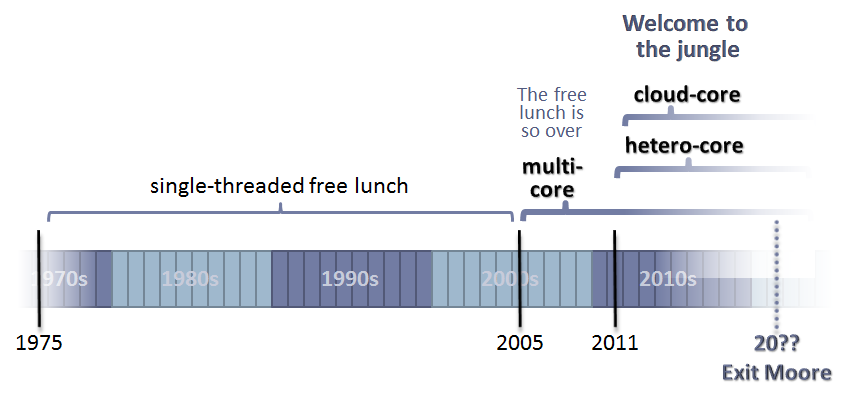
\includegraphics[width=0.9\textwidth]{img/free_lunsh.png}
\caption{Illustration of several transitions currently taking place in the computer industry. \todo{Site Herb Sutter - Welcom to the jungle http://herbsutter.com/welcome-to-the-jungle/}}
\label{fig:jungle}
\end{figure}

Around the same time as CPU manufactures hit the frequency wall, people started experimented with programmable shaders which recently had been introduced in the field of graphics programming. The graphics processing pipeline had previously been a fixed function pipeline, where e.g. vertices and texture coordinates where fed to the graphics processing unit (GPU) in one end and a rasterized rendered image was outputted in the other. What programmable shaders  introduced was the ability to replace some steps in the fixed-function pipeline with custom computations. This made it possible to utilize the GPU for other tasks than just rendering graphics. The graphics pipeline could for instance be hacked to evaluate a differential equation over grid defined by graphics primitives\todo{cite Seland et al.}. The rationale behind this exploration was that hidden in the GPU was processing power an order of magnitude larger than what the CPU could provide at the same time. Actually, at this time, the GPU had already gone multi-core, driven by the increasing demand for realistic computer games. Multiple cores was somewhat easier to achieve with the GPU since the rendering problem is inherently parallel. The pixels in the rendered image can be calculated in any order, and one pixel is therefore an concealed unit which the GPU scheduler is free to issue at any time to whatever core that is available. It it is also much less costly to switch between a pixel-thread for the GPU then a program thread for the CPU. Since there was only one program running on the GPU, the fixed function pipeline, GPU designers had a good idea of how the program would execute, and could therefore skip advance feature as predicting execution paths and different levels of data caching.  The released silicon was used to make more cores. 

It is common to say that a CPU has few but advance generic cores, and the GPU has many but simple cores.

Three eras at the same time: Multi-core, Heterogeneous-cores, and Cloud-cores.

Early gpgpu programming required expert knowledge about graphics and the remaining fixed funtions in the pipeline. New programming languages where needed. OpenCL and CUDA. C++ AMP.

Architecture and how to program. See Paper II.

About theoretical FLOPS: Note that these are theoretical numbers and the actual throughput typically is algorithm dependent.

Compare CPU and GPU ALUs.

Add sentence about siemens and supersonic imagine scanners. They use GPUs? What does this mean? FPGAs and ASICs.

\begin{figure}
\centering
\subfigure[Threads, blocks and grid]{
	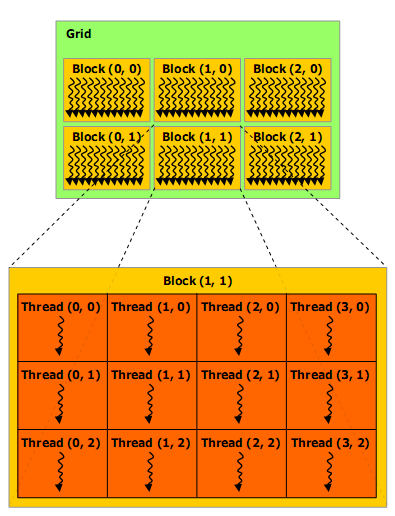
\includegraphics[width=0.4\textwidth]{img/cuda_threads.png}
}
\subfigure[Kernel]{
	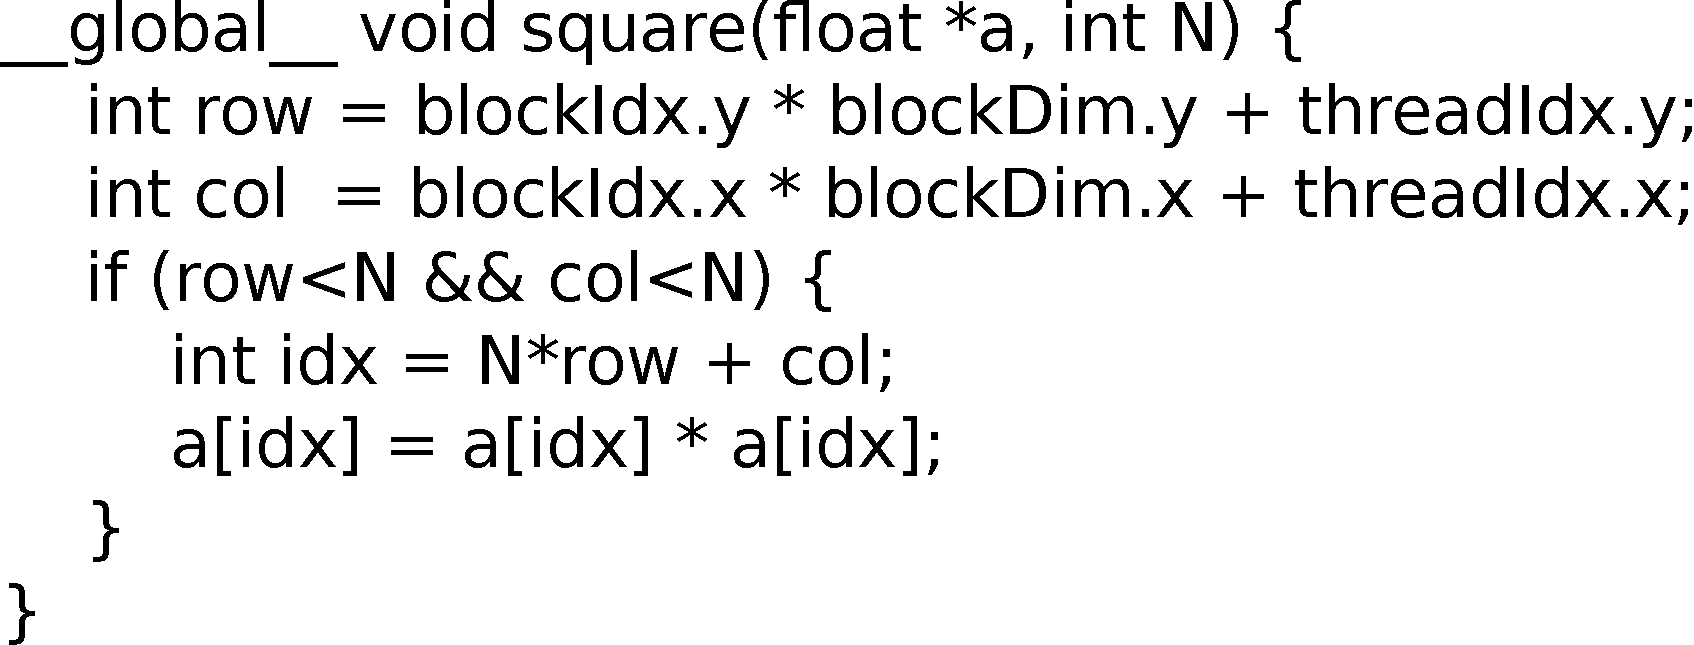
\includegraphics[width=0.5\textwidth]{img/kernel.pdf}
}
\caption{Depicts how GPU threads are grouped into blocks and arranged in a grid. One thread runs a copy of a kernel function, in this example an element-wise matrix square operation.}
\label{fig:gpu_grid}
\end{figure}

\section {Medical ultrasound imaging}\label{sec:ultrasound}
Ultrasound imaging encompasses technology which generates images based on sound whose frequencies we can not hear. For medical ultrasound imaging frequencies above 2 MHz are typically used.

Small section about heart anatomy.

\begin{figure}
\centering
\subfigure{
	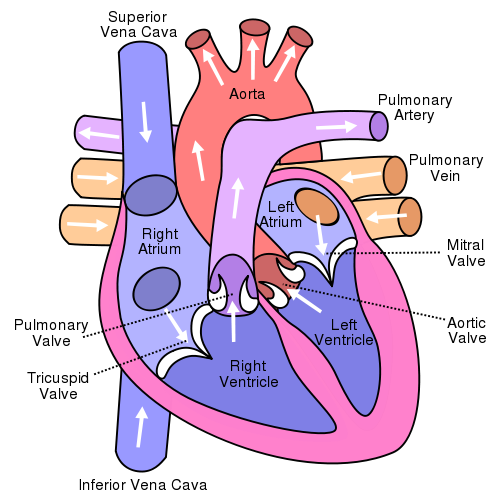
\includegraphics[width=0.47\textwidth]{img/Diagram_of_the_human_heart.png}
}
\subfigure{
	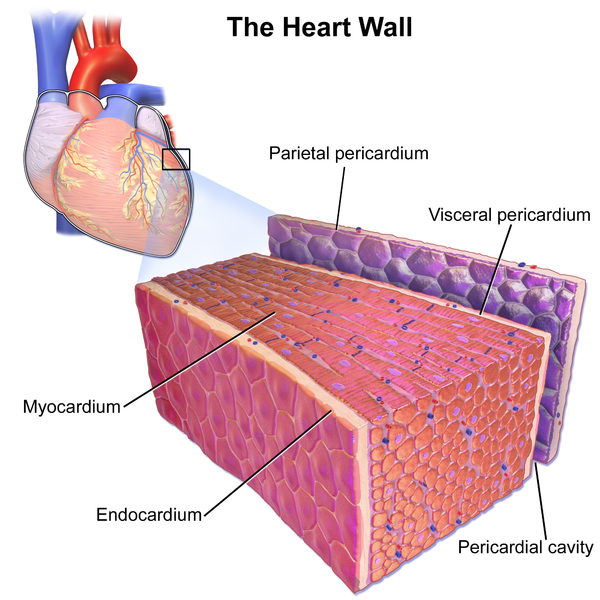
\includegraphics[width=0.47\textwidth]{img/HeartWall.png}
}
\caption{Overview of the human heart. Illustrations from wikipedia.org.}
\label{fig:human_heart}
\end{figure}

Typical probes, scan sequences, resolution and sampling.

Key selling points of ultrasound imaging: cost, safety and real-time user interaction.

One sentence about speckle tracking.
							
\subsection{Basic beamforming}

Delay and sum. Apodization. (See intro to Paper II or III).
Time v.s. phase delays.

\subsection{Adaptive Beamforming}\label{sec:adaptbf}

\begin{figure}[t!]
\subfigure[Delay-and-sum]{
	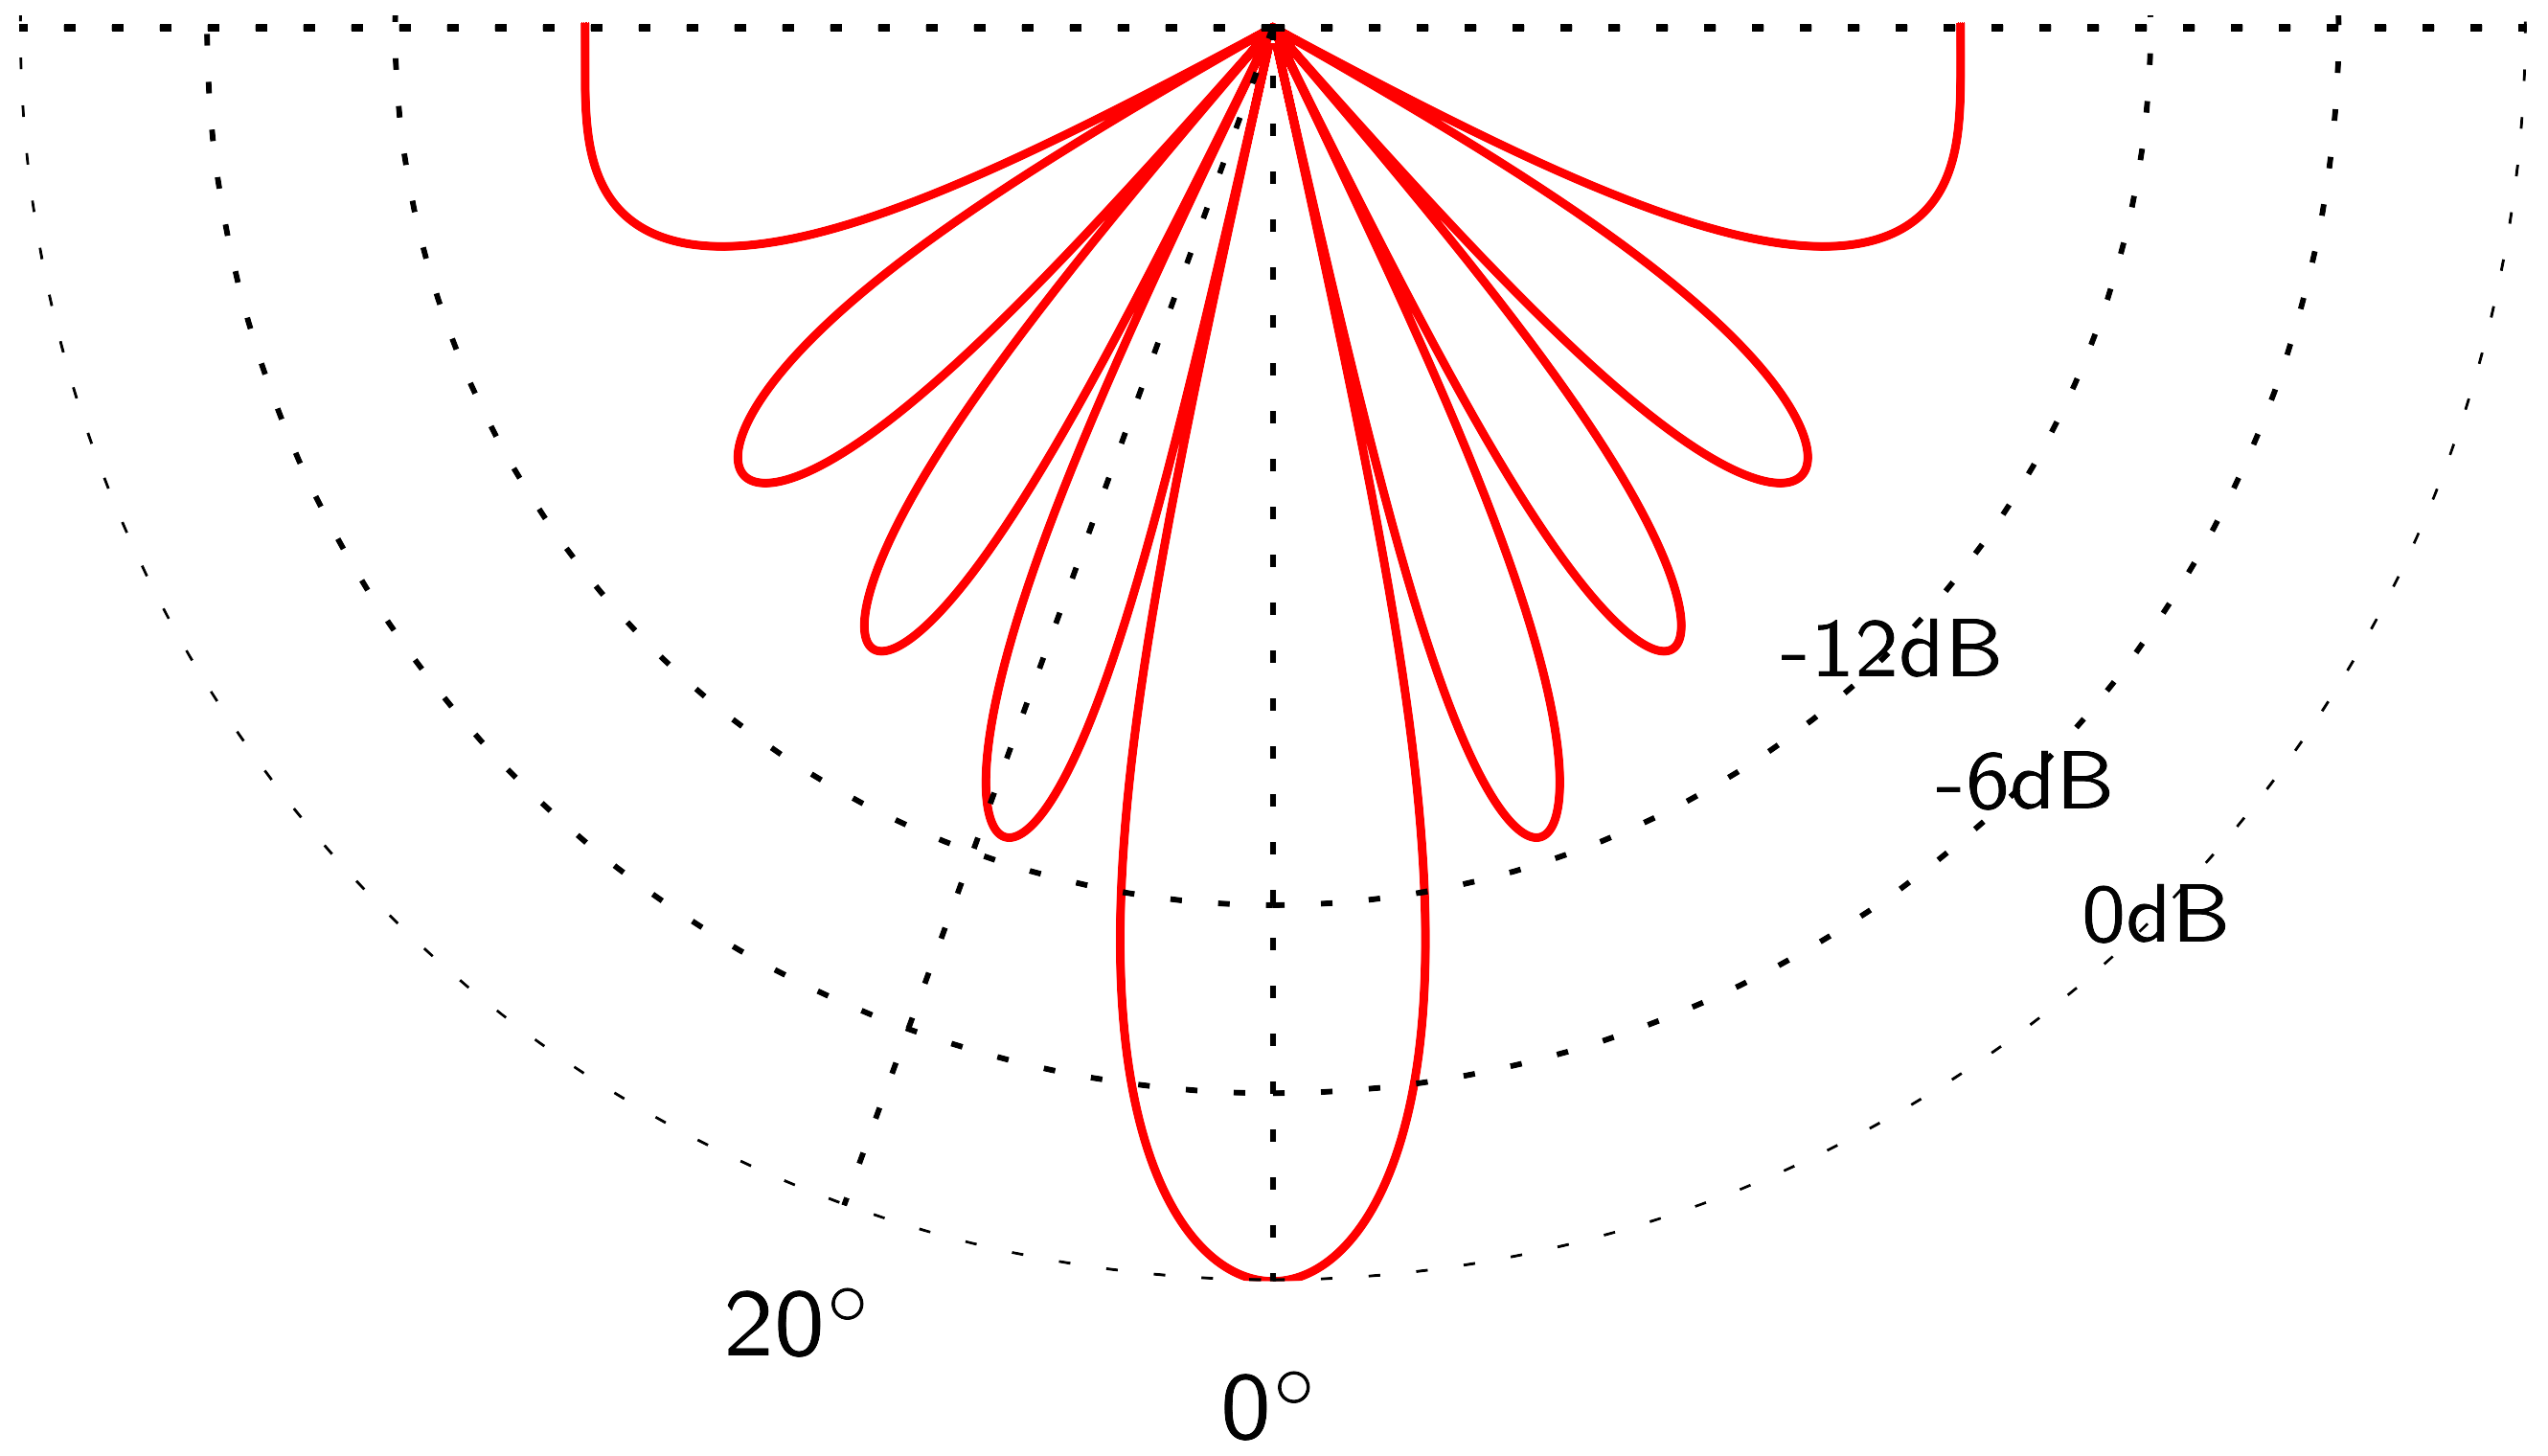
\includegraphics[width=0.47\textwidth]{img/scenario_das_resp2.png}
}
\subfigure[Capon]{
	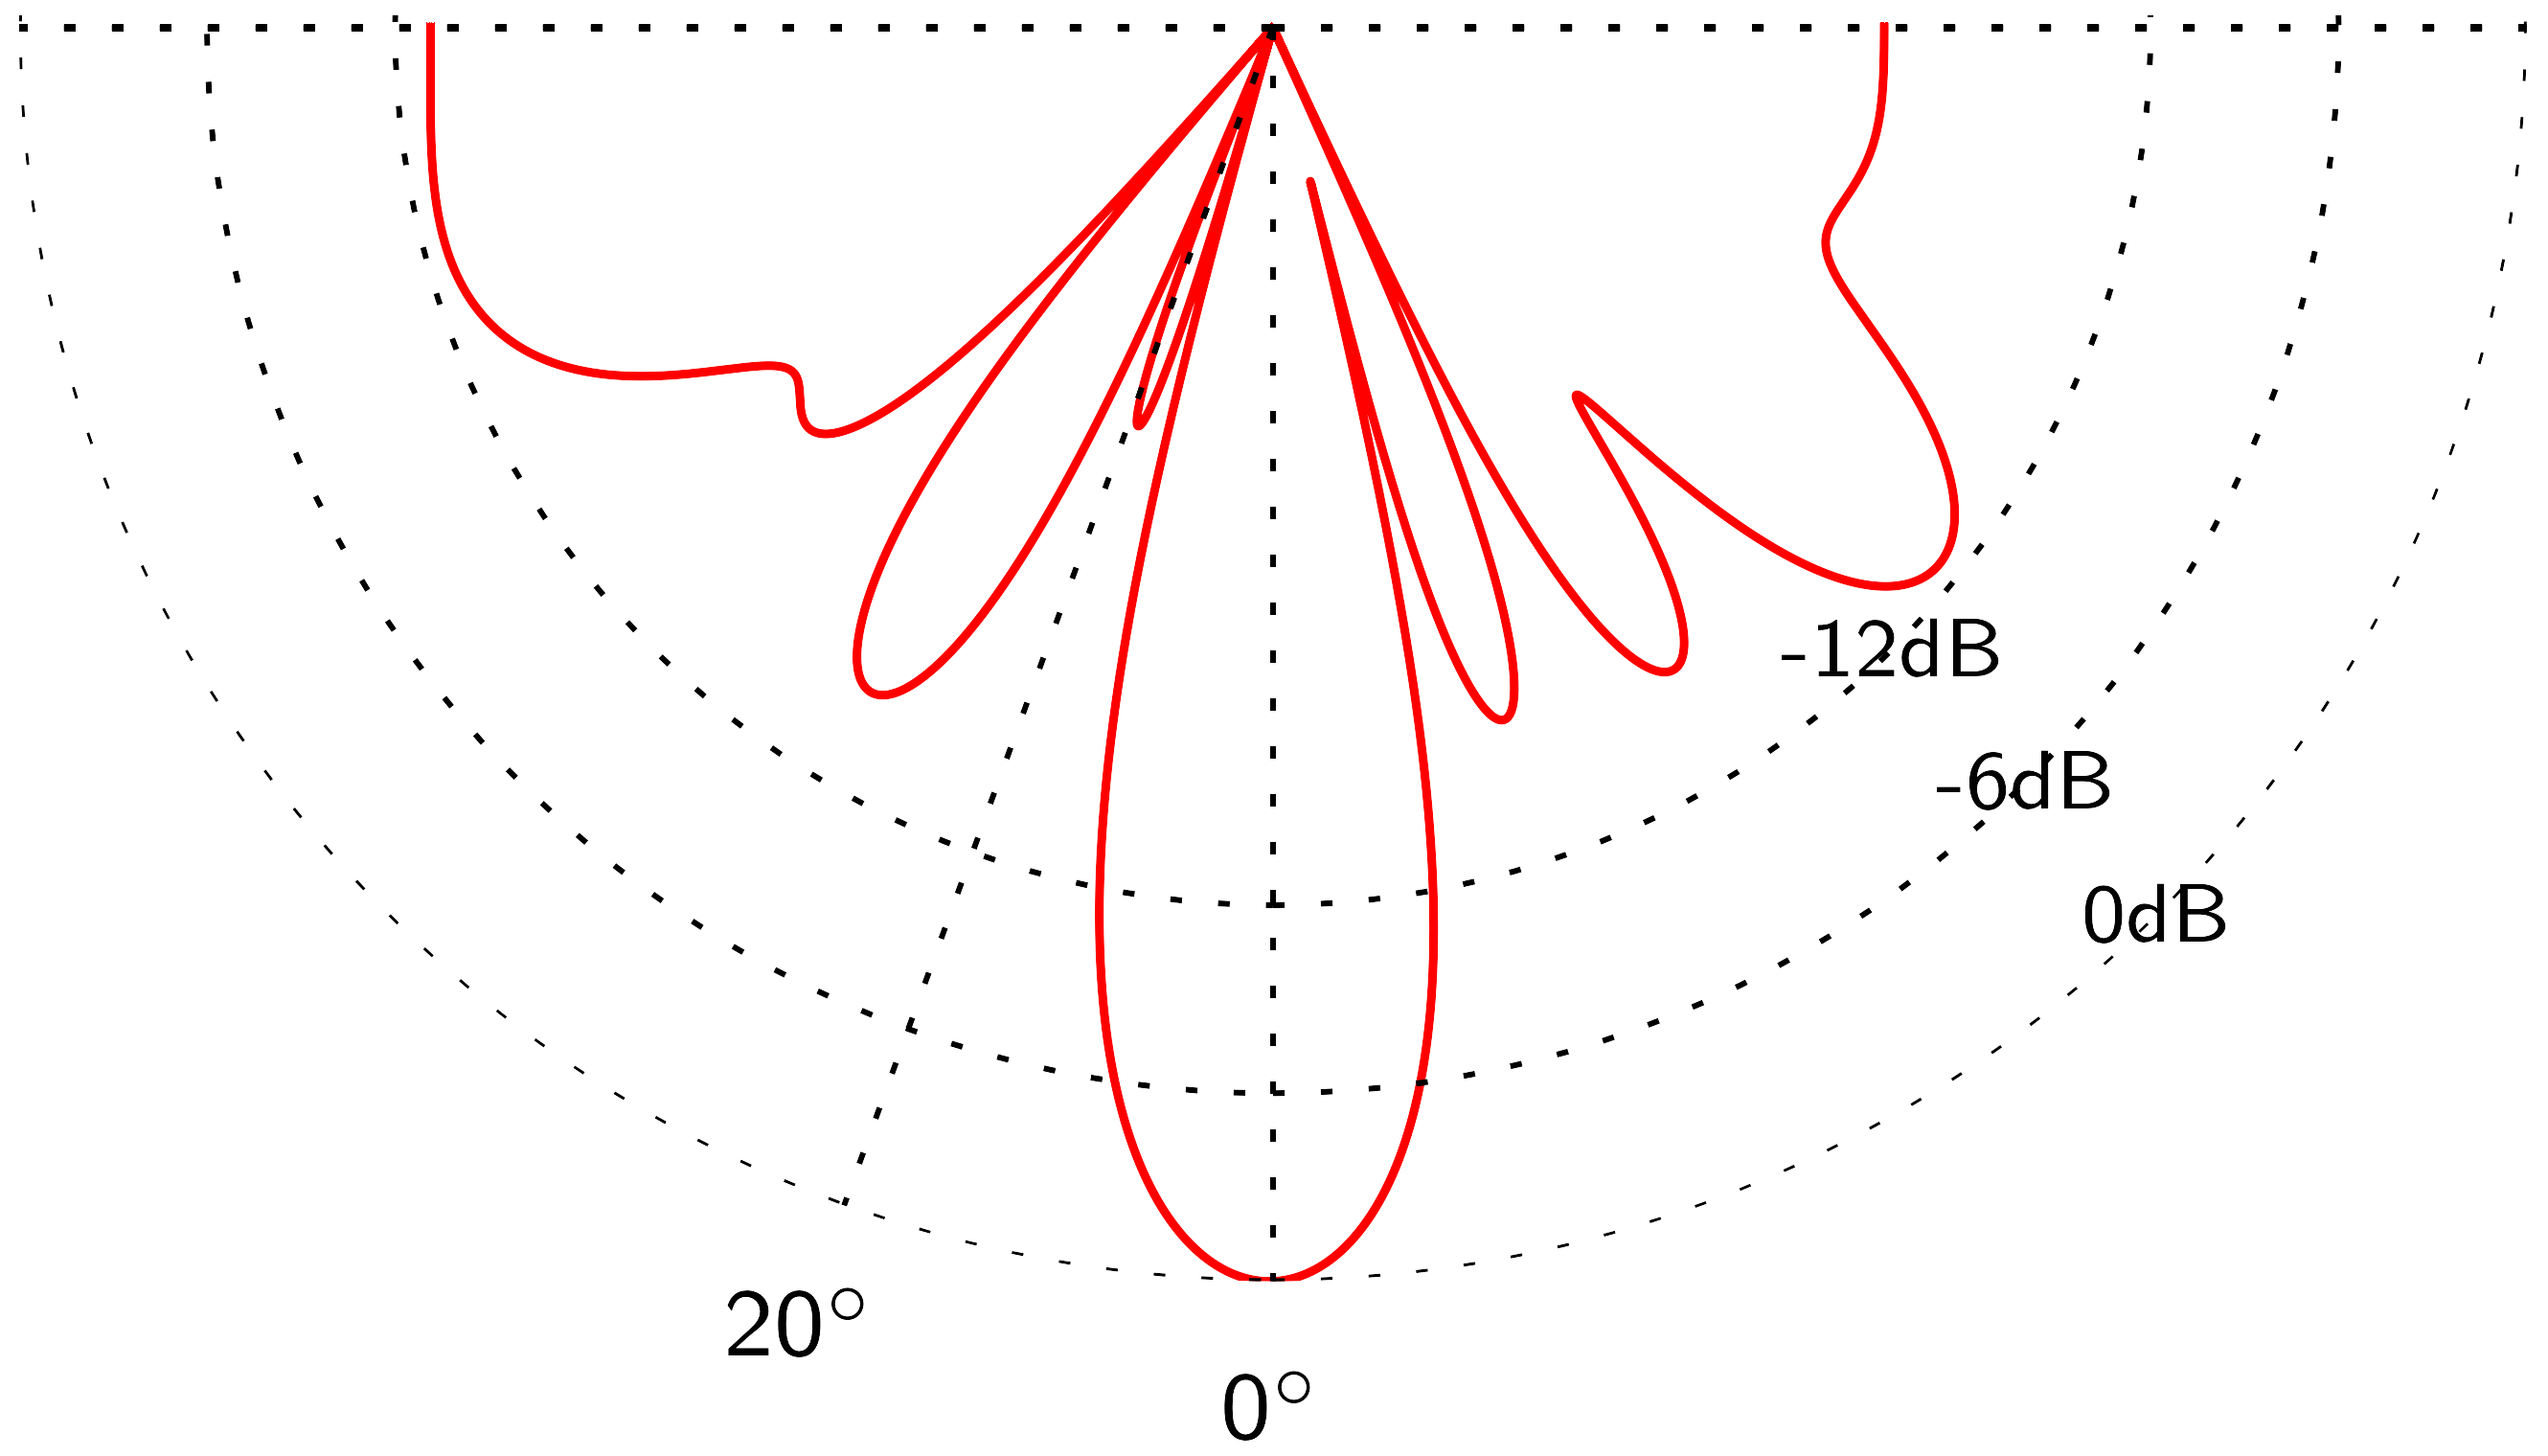
\includegraphics[width=0.47\textwidth]{img/scenario_mv_resp2.png}
}
\caption{Array beam pattern with uniform and Capon weights. An interfering source is located at 20 degrees.}
\end{figure}

Capon beamforming\footnote{The name ''Capon beamformer'' is due to work by J. Capon \todo{add citation} on seismic arrays \todo{Move to background.}} or minimum variance beamforming.

Intro to adaptive beamforming. List other variants (LCA, beamspace, Eigen space etc.). 

Beamspace data is typically refers to the polar grid that cardiac ultrasound data is located in prior to scan conversion. In combination with the Capon beamformer, beamspace refers to the K-space representation of the impinging signals (hence the \nom{FFT}{Fast fourier transform} of the channel data). 

Not phase aberration correction.

Add section about the computationally complexity. How many flops are required per rx-beam etc...

Add section about how to present data (max v.s mean etc.)
						
\subsection{Shift invariance}

\section{Volume rendering}\label{sec:volren}

Get section from master theses. Ray casting and opacity functions.

\begin{figure}
\centering
\subfigure[Ray-casting]{
	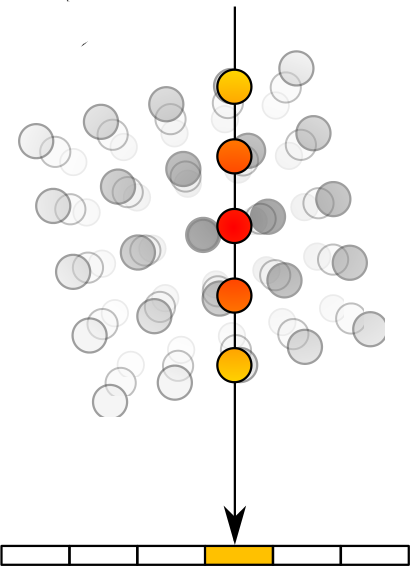
\includegraphics[width=0.4\textwidth]{img/Volumeraycasting.png}
}
\subfigure[Opacity transfer function]{
	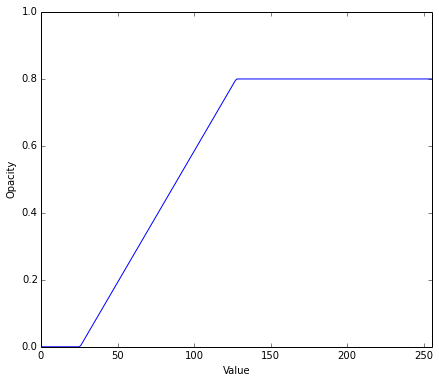
\includegraphics[width=0.5\textwidth]{img/otf.png}
}
\caption{.}
\label{fig:vr}
\end{figure}

\subsection{Adaptive volume rendering}

Visibility driven visualization.

\section{Field simulations}\label{sec:field}

Small chapter about different simulation tools (See hos paper).
			
\endinput

\newpage\addcontentsline{toc}{section}{References}
\putbib[bibBackground]
\end{bibunit}

%\setcounter{section}{0}
%\setcounter{chapter}{1}

%%%% CHAPTER 1 %%%%
\begin{bibunit}[ieeetr]
\CustChapter{Introduction} 
%\addcontentsline{toc}{chapter}{Introduction}
\runningtitle{Introduction}
\section{Motivation}
A rapid development in computer game technology and accompanying programming languages have recently provided researchers with small personal super computers, comprised in a single graphics card (\nom{GPU}{Graphics processing unit}). The latest graphics cards\footnote{As of January 2014.} from both \nom{Nvidia}{Graphics card producer} and \nom{AMD}{Graphics card producer} provide close to 6 T\nom{FLOPS}{Floating point operations per second} single precision and 1.5 TFLOPS double precision computations. For double precision this is more than the worlds most powerful supercomputer could provide in 1998.

This immense rise in computational power and improved programmability are currently changing how ultrasound imaging systems are designed. Algorithms which previously had to be implemented in hardware for performance reasons can now be implemented in software. And algorithms, either too complicated or costly to implement in hardware, and where a software implementation was thought to be too computationally heavy for real-time use, becomes realizable. It is clear that high-performance programmable processors, like the GPU, already have and will continue to make future ultrasound imaging systems more flexible, cheaper to produce, and equipped with even more cutting-edge processing.

The Capon beamformer  is a good example of an algorithm which has been highly studied for the last decade for the application of medical ultrasound imaging, but where the number of calculations was thought to be too high for real-time processing to happen any time soon. No wonder, to achieve real-time processing for e.g. cardiac ultrasound imaging, an effective processing rate of around 100 MFLOPS is required. This number, as explained in Section \ref{sec:adaptbf}, also grows with larger subarrays, an increasing number of samples, and higher frame rates.  Nevertheless, with modern GPUs, these levels of processing are finally available within a single card. When researchers are exploring new algorithms for ultrasound imaging it is therefore important to keep the architecture of parallel accelerators in mind. If a new complex algorithm is suppose to run in real time it needs to fit the programmable and parallel pipeline of modern ultrasound scanners.

\section{Aims of study}
The overall aim of this study has been to investigate the possibility of utilizing GPUs for advanced processing in an ultrasound imaging system. 

Main focus have been the Capon beamformer, and the problem of making this computationally intense algorithm available for real-time ultrasound imaging (\textbf{Paper\,I} and \textbf{II}). However, two additional methods were also explored. The first is adaptive visualization of cardiac ultrasound volumes (\textbf{Paper\,IV}) and the latter is simulation of dense ultrasound pressure fields (\textbf{Paper\,V}). Both share the property of being computationally complex, but on the other hand they consist of many independent computations which makes them perfectly suited for parallel GPU acceleration.

Well on my way into the project, when a real-time Capon beamformer was realized, and loops of images for the first time were processed at real-time frame rates, new issues where discovered and had to be solved. This led to a more theoretical study of the Capon beamformer in \textbf{Paper\,III}, with special attention on how to obtain high lateral resolution while preserving the important shift-invariant property of ultrasound imaging. Shift-invariant behavior is crucial if the method is ever to be applied for live scanning. 

%\subsubsection{Accelerate the Capon beamformer to facilitate real time imaging}

%\subsubsection{}

\section{Summary of papers}

\subsection{Paper\,I}
\textbf{An Optimised GPU Implementation of the MVDR Beamformer for Active Sonar Imaging}\\
J.\:I.\:Buskenes, \textbf{J.\:P.\:\AA{}sen}, C.-I.\:C.\:Nilsen and A.\:Austeng\\
{\it IEEE Transactions on Oceanic Engineering, submitted.}\\\\
The first paper describes in details how the Capon beamformer was mapped to GPU architecture. Even though the paper is written within the field of active \nom{sonar}{SOund Navigation And Ranging (usually under water)} imaging, the depicted implementation is applicable to a vast range of active imaging systems. A similar discussion for cardiac ultrasound imaging can be found in \textbf{Paper\,VI}.  Active sonar imaging typically differs from medical ultrasound imaging by a lower real-time requirement and fewer array elements. This makes it somewhat easier to reach the goal of real-time processing. 

The estimation of the spatial covariance matrix receives special attention in this study. In previous literature on Capon beamforming the matrix inversion has always been regarded as the most computationally complex step. In this paper we show that estimation of the sample covariance matrix is actually the most complex part when spatial and temporal smoothing with common parameters are included. It is then shown how the arithmetic complexity of this estimation process can be reduced from cubic to square. Finally, an in-depth analysis of the arithmetic throughput on multiple platforms is given. Despite our effort, the number of effective FLOPS is only 4 \% and 14 \% of the theoretical throughput of the target GPU for the matrix equation solver and covariance estimator respectively. Still, the reported throughput of 1 Mpx/s on a high-end GPU is enough to provide real-time processing for common sonar scan sequences.

\subsection{Paper\,II}
\textbf{Implementing Capon Beamforming on a GPU for Real-Time Cardiac Ultrasound Imaging}\\
\textbf{J.\:P.\:\AA{}sen}, J.\:I.\:Buskenes, C.-I.\:C\:Nilsen, A.\:Austeng and S.\:Holm\\
{\it IEEE Transactions on Ultrasonics, Ferroelectrics, and Frequency Control, vol. 61, no. 1, pp. 76-85, Jan. 2014.}\\\\
The second paper aims at implementing real-time Capon beamforming for cardiac ultrasound imaging. Achieving this will facilitate further study of the method's \textit{in vivo} performance. This is something which has been stated as further work in many publications on Capon beamforming for medical ultrasound imaging the past decade. In \textbf{Paper\,I} arrays with no more than 32 elements were investigated. A linear array for cardiac ultrasound imaging typically has 64 or more elements. In \textbf{Paper\,VI}, which is summarized in \textbf{Paper\,II}, it is shown that our implementation from  \textbf{Paper\,I} does not reach the level of throughput required for real-time Capon beamforming of cardiac ultrasound imaging. The matrices that have to be inverted become to large, and the frames that need to be processed per second are too many.

In this paper, to reduce the matrix size, it is taken advantage of the beamspace version of the Capon beamformer (\nom{BS-Capon}{Beamspace capon beamforming}), which is implemented on the GPU. For parameters previously derived to give similar performance for BS-Capon and element-space Capon (\nom{ES-Capon}{Element space capon beamforming}), we show that real-time BS-Capon beamforming is feasible for cardiac ultrasound imaging. The reported processing throughput is able to keep up with the acquisition frame rate in a typical cardiac ultrasound imaging system equipped with 64 and 96 element linear arrays.  \textbf{Paper\,II} and \textbf{VI} also presents, for the first time, videos where the ES-Capon and BS-Capon beamformer have been applied on loops of simulated and \textit{in vivo} medical ultrasound images.

\subsection{Paper\,III}
\textbf{Capon Beamforming and Moving Objects - An Analysis of Lateral Shift-Invariance}\\
\textbf{J.\:P.\:\AA{}sen}, A.\:Austeng and S.\:Holm\\
{\it IEEE Transactions on Ultrasonics, Ferroelectrics, and Frequency Control, submitted.}\\\\
In the third paper we study the shift-invariant property of an imaging system based on the Capon beamformer. As mentioned, shift-invariant imaging is essential if the method is ever to be adopted. The paper was written based on observations of aliasing artifacts when imaging bright point scatterers \textit{in vitro} and in simulations. The point scatterers were observed to twinkle like stars in the sky. In earlier work on Capon beamforming for medical ultrasound imaging the real-time nature of ultrasound imaging has often been ignored, and a large degree of oversampling on transmit might have been applied without being clearly stated. Oversampling on transmit is not an option if the imaging modality is used to image rapidly varying objects. Smooth presentation of probe motion is equally important since real-time user interaction is one of the key selling points of ultrasound imaging. The frame rate should therefore be higher than 10 frames per second.

Further it has been investigated how the Capon beamforming achieves its super resolution, and how this makes it highly sensitive to differences between the assumed steering vector and the signal propagation vector. Earlier work, focusing on single images, has typically referred to this effect as speed-of-sound errors, however, it also comes naturally into play when objects moves from frame to frame and the beam density is insufficient. With a narrowband and farfield model it is shown that the Capon beamformer suffers from beam-to-beam gain variations as large as 27 dB for parameters previously used to obtain high resolution medical ultrasound images.  To obtain the same lateral gain variations as with \nom{DAS}{Delay-and-sum beamforming} beamforming, 25 times oversampling is shown to be required. For broadband nearfield simulations the same gain variations are observed. Finally we show that the gain variation can be reduced, hence improved shift-invariance, by oversampling on receive using phase rotation steering. This is achieved without affecting the acquisition frame rate and with a minor increase in computational complexity. The method is successfully applied on simulations and \textit{in vitro} phantom data.

\subsection{Paper\,IV}
\textbf{Adaptive Volume Rendering of Cardiac 3D Ultrasound Images - Utilizing Blood Pool Statistics}\\
\textbf{J.\:P.\:\AA{}sen}, E.\:Steen, G.\:Kiss, A.\:Thorstensen and S.\:I.\:Rabben\\
{\it Proc. SPIE Medical Imaging 2012, vol. 8320, pp. 832008.}\\\\
The fourth paper propose an adaptive volume rendering method based on statistics derived from the blood pool of the left ventricle. Noise located in the blood pool tends to occlude cardiac tissue when rendered in 3D, and is often impossible to remove by adjusting global rendering parameters. This because ultrasound signals have high variability within blood as well as high variability within tissue, even when heavily smoothed. Delineation of the blood pool is done by a state estimation algorithm, capable of tracking the endocardium in real time. The final visualizations are compared, with respect to location of tissue, by using a state-of-the-art endocardium segmentation tool. The paper presents both quantitative and qualitative results supporting the method's improved capabilities of reducing tissue dropouts and spurious structures inside the blood pool, leading to a maximized amount of visible endocardium tissue. The proposed method is implemented on a GPU with real-time frame rates as the result. This results shows that with modern GPUs it is possible to add more advanced visualization to an ultrasound imaging system and still have real-time performance.

\subsection{Paper\,V}
\textbf{Huygens on Speed: Interactive Simulation of Ultrasound Pressure Fields}\\
\textbf{J.\:P.\:\AA{}sen} and S.\:Holm\\
{\it Proc. IEEE Ultrasonics Symposium 2012, pp. 1643-1646.}\\\\
The fifth paper presents an interactive simulations tool capable of simulating dense pressure fields from ultrasound arrays in real time. Simulation tools are heavily used by researchers in order to test out new algorithms and to deduce the performance of new array designs prior to manufacturing. However, dense simulations involve extensive calculation and computational time. With the presented simulator we aim at reducing the time needed for calculating pressure fields by means of GPU acceleration. The tool is based on Huygens' principle which describes diffraction caused by a slit as the superposition of several point sources located inside the opening. Thus, the simulator works by accumulating the contribution from a collection of point sources in a set of observation points. How the source and observation points are laid out is left for the user to decide. Point sources positioned along a line will for instance simulate an ultrasound array. The simulator is linked with both a Paint-like interface for interactive drawing of arrays, and a Matlab interface for precise scripting of array configurations. The main contributions in this paper is the increased performance of the GPU implementation compared with a CPU and Matlab\footnote{The Ultrasim toolbox \todo{add citation}} version. Second, the paint-like interface provides a neat way of demonstrating array beamforming principle in real time. We believe this to be of great value both for array designers and teachers.

\section{Main contributions}
The main contributions of this thesis are:
\begin{enumerate}
\item a GPU implementation of the Capon beamformer.
\item a GPU implementation of the beamspace Capon beamformer.
\item that real-time beamspace Capon beamforming is achieved for cardiac ultrasound imaging.
\item the first investigation of Capon beamforming applied on multiple frames in medical ultrasound imaging (simulated, \textit{in vitro}, and \textit{in vivo}).
\item an investigation of shift-invariance when the Capon beamformer is applied on consecutive frames.
\item a method for improved shift-invariance of the Capon beamformer when applied to medical ultrasound imaging.
\item a method for reduced blood-pool noise in volume renderings of cardiac ultrasound volumes.
\item a GPU implementation of this adaptive volume rendering method.
\item a GPU implementation of simple Paint-like simulation tool for rapid visualization ultrasound pressure fields.
\end{enumerate}
In addition, the thesis provides several discussions on how to utilize the GPU to accelerate advanced ultrasound imaging algorithms. 

\section{Discussion and future work}
Even with all our effort in \textbf{Paper\,I} we were only able to achieve a fraction of the maximum throughput of the target GPU. This result shows how hard it is to reach the theoretical level of throughput, and that how close one can get is highly algorithm depended. It might be ways to improve on these numbers, but both the solver and covariance estimation step consist of several points where fine granular synchronization and serialized instructions are needed. This will restrict even the most fine tuned implementation from reaching the maximum throughput of the GPU. An interesting observation can be found in Fig.\,10 of \textbf{Paper\,I}. Here we see how the achieved throughput of the covariance estimation kernel is more than three times higher than the theoretical throughput of a modern, high-end, \nom{CPU}{Central processing unit}. This clearly shows the benefit of modern GPU computing.  Solving was performed by a batched Gauss Jordan solver implemented by Nvidia. In our work we focused on the covariance estimation step, and did not try to beat Nvidia at home. Nevertheless, with the measured throughput in mind, a natural next step would be to analyze the current solver, and figure out if any further optimization is possible. Since the sample covariance matrix is hermitian, a solver based on Cholesky decomposition might also help to improve the solver's throughput.
\\\\
In \textbf{Paper\,II} we focused on achieving real time Capon processing for cardiac ultrasound by implementing the BS-Capon beamformer on a GPU. However, we also present the first medical ultrasound loops processed with ES- and BS-Capon beamforming.  The paper does not provide any detailed evaluation of the method's \textit{in vivo} performance. Yet, initially it has been proven hard to transfer all results obtained in simulations to \textit{in vivo} images. The improvements seen are minimal, especially with the number of calculations in mind. The beamformers are clearly able to decrees the lateral width of lateral point scatterers and thin structures \textit{in vivo}, and to sharpen step edges. On the other hand, the overall contrast is visually not improved and sometimes it is worse (Fig.\,6b of \textbf{Paper\,II}). Since the Capon beamformer only affect directional noise, it is clear that contrast will get worse in low \nom{SNR}{Signal-to-noise ratio} situations when signal cancellation occurs. The oversampling approach presented in \textbf{Paper\,III} might improve on this, but it will only reduce signal cancellation if the phase shifts across the aperture are close to linear and small. Another issue is that bright points with a wide lateral profile exhibits better visual contrast when surrounded by speckle noise than points with narrow lateral profiles. In future work a detailed investigation of why some results, especially the contrast, obtained in simulations are not transferable to \textit{in vivo} needs to be performed. It will also be crucial to show larger improvements \textit{in vivio} than what is presented in \textbf{Paper\,II}. Both to justify all our computations, and to show an image which has both highly improved resolution and contrast. As pointed out at the end of \textbf{Paper\,II}, cardiac ultrasound imaging might not be the best modality for Capon beamforming. Cardiac ultrasound imaging was mainly selected because it is the medical ultrasound modality which requires most calculations per second. An application where the focus is detection of closely spaced point targets, might be better suited. A better suited adaptive beamformer for cardiac applications might be the low-complexity adaptive beamformer (\nom{LCA}{Low complexity adaptive (beamformer)} beamformer), where the Capon optimization problem is applied on a set of predefined windows. This method has linear complexity and shares many properties with the Capon beamformer. If only minor improvements are obtained, it would be easier to ignore this fact if the algorithm is less computationally costly. Finally, it would also be interesting to see how the Eigenspace-based Capon beamformer performs on cardiac images, and how its absence of a distortionless criterion will influence the image spatially and temporally. The work in \textbf{Paper\,II} made it clear that interesting findings are done when users are able to watch the temporal behavior of an algorithm. This led us to the work of \textbf{Paper\,III}. 
\\\\
In \textbf{Paper\,III} we investigate the inherent self nulling involved with Capon beamforming, and how this effect comes naturally into play when the beamformer is subjected to linear steering vector errors caused by lateral undersampling. These errors are naturally reduced when the lateral sampling is increased. This simple observation is something which has been missing in the literature on Capon beamforming for medical ultrasound imaging. The reason could be ignorance or its possible negative impact on imaging frame rate. A lack of studies where Capon beamforming is performed on consecutive frames might also explain the lack of comments. Fortunately, as shown in \textbf{Paper\,III}, it is possible to maintain the same frame rate as with DAS beamforming by applying oversampling on receive using a set of steering vectors (phase delays). It also turns out that more matrix inversions are not needed either. Oversampling on receive will, however,  increase the penalty of applying post-processing, like filtering,  on scan-grid data. %The time taken to convert data from a polar scan grid to a Cartesian display grid will also increase. The Cartesian grid should also have high resolution in order to preserve the un-sharpening introduced by Capon beamforming. 
As just mentioned in the discussion of \textbf{Paper\,II}, reduced signal cancellation should prevent contrast from degrade to less than the contrast obtain with DAS. It will, however,  not correct for signal cancellation caused by phase aberrations. At best it will correct for the linear term introduced by the aberrator if the term is small.
With improved shift-invariance it will also be interesting to see if high resolution beamforming could act as a post-processing step for other algorithms. For example to increase the precision of speckle and edge tracking. In the case where the image is generated for post processing it does not need to be visually pleasant anymore, as long as signal cancellation is avoided. Good looking speckle, or DAS-like speckle, has been the driving force behind many of the robustification techniques and the default parameters seen in the literature. Hence, more aggressive parameters might be used if the image produced is intended as input to another algorithm and not for the human eye.
\\\\
%Objections to \textbf{Paper\,IV} includes its inherent chicken-or-egg dilemma. The visualization is adjusted based on the data acquired by a user. The user sees the visualization and adjust scanning based on the visual input. This recursive behavior suggest that the method is best suited for post-processing when data has been recorded and saved. 
%Does data need to be saved in order to perform tracking?
One limitation of the algorithm described in \textbf{Paper\,IV} is its dependence on a successful tracking. If the tracking fails the proposed method will fail.  Another issue is the view-dependent visibility, where an object could become visible or disappear while rotating or if the local statistics change a lot during the cardiac cycle. Even if the method successfully removes noise, this means that the rendering will become non-intuitive to interact with and unrealistic to watch. However, the method could still be used to clean up still images of standard cardiac views. The paper does also propose an interesting method for automatic tuning of rendering parameters. Figure 3d in \textbf{Paper\,IV} actually shows that an optimal threshold could be found based on global and not only local statistics. Even though the visualization based on global statistics has more errors, with respect to endocardium visibility, the tuning of the opacity function is still fully automatic if an iterative search for the minima in Figure 3d is performed. A global opacity transfer function will assure a rendering which are realistic, but it will still be dependent on a successful tracking for the auto-adjustment to work. An automatically tuned opacity function based on global statistics combined with an improved smoothing scheme is likely to be better suited for cardiac ultrasound imaging than a local opacity transfer function. A local opacity transfer function is just to extreme to be clinically robust. It would also be interesting to see if statistics based on the window selected by the Capon or the LCA beamformer could be utilized to adjust the opacity. It should also be possible to use this statistic as input to image filtering. An adaptively selected window will be symmetric in homogeneous regions and left-right shifted close to tissue interfaces. In that way we can apply less filtering and higher opacity on edges. If this will be different than just looking at neighboring pixels in a smoothing filter is to be seen.
\\\\
The fifth paper stands out from the other papers by not dealing with an adaptive processing technique. It is still, however, centered around the topic of implementing algorithms for ultrasound imaging on GPUs. Ultrasound simulations are typically used for research and sometimes also to pre-calculate configurations of a given scan sequence, for instance to achieve a certain pressure in a given area. The continuously growth in computational power will, in the future, make it possible to evaluate a scan sequence on the fly, removing the need for lookup tables. Estimation of the mechanical and thermal index could also be improved. Achieving higher processing speed for an excising algorithm by implementing it on a new architecture is not academically relevant in its own. It has to be combined with either a good analysis of what special adjustments that had to be made to the algorithm in order for the increase to happen or a suggestion of how to utilize the speed gained. These are points we have tried to answer in both \textbf{Paper\,I}, \textbf{II},  \textbf{IV}, and \textbf{V}.  In \textbf{Paper\,V} the increased speed made an interactive ''Paint-program'' feasible. As of January 2014 the simulator has been download 200 times and counting. It also has close to a "whopping" 1000 views on youtube. 
\\\\
Finally it is worth mentioning that the code for both the Capon beamformer\footnote{github.com/jpaasen/cos} and the ultrasound field simulator\footnote{github.com/jpaasen/hos} have been made open source and is available on github. 
\endinput
\newpage\addcontentsline{toc}{section}{References}
\putbib[bibIntroduction]
\end{bibunit}

\setcounter{chapter}{0}

%%%% Paper 1 %%%%
\begin{bibunit}[ieeetr]
\CustChapterPaper{An Optimised GPU Implementation of the MVDR Beamformer for Active Sonar Imaging}
\runningtitle{GPU MVDR Beamformer for Active Sonar Imaging}
\authors{
	Jo Inge Buskenes$^{1}$, 
    	\textbf{Jon Petter \AA{}sen}$^{2}$, 
    	Carl-Inge C. Nilsen$^{1}$ and
    	Andreas Austeng$^{1}$
} 
{
	$^{1}$Department of Informatics, University of Oslo, Oslo, Norway\\
    	$^{2}$Medical Imaging Lab (MI-Lab), Norwegian University of Science and Technology, Trondheim, Norway
}
\noindent \textit{IEEE Transactions on Oceanic Engineering, submitted}
%\newpage\input{./CaponSonarGPU/CaponSonarGPU}
%\newpage\addcontentsline{toc}{section}{References}
\putbib[bibCaponSonarGPU]
\end{bibunit}


%%%% Paper 2 %%%%
\begin{bibunit}[ieeetr]
\CustChapterPaper{Implementing Capon Beamforming on a GPU for Real-Time Cardiac Ultrasound Imaging}
\runningtitle{GPU Capon Beamformer for Cardiac Ultrasound Imaging}
\authors{
	\textbf{Jon Petter \AA{}sen}$^{1}$,
    	Jo Inge Buskenes$^{2}$,  
    	Carl-Inge C. Nilsen$^{2}$,
    	Andreas Austeng$^{2}$ and
    	Sverre Holm$^{1,2}$
} 
{
	$^{1}$Medical Imaging Lab (MI-Lab), Norwegian University of Science and Technology, Trondheim, Norway\\
    	$^{2}$Department of Informatics, University of Oslo, Oslo, Norway
}
\noindent \textit{IEEE Transactions on Ultrasonics, Ferroelectrics, and Frequency Control, vol. 61, Jan 2014}
%\input{./CaponCardiacGPU/CaponCardiacGPU}
%\newpage\addcontentsline{toc}{section}{References}
\putbib[bibCaponCardiacGPU]
\end{bibunit}


%%%% Paper 3 %%%%
\begin{bibunit}[ieeetr]
\CustChapterPaper{Capon Beamforming and Moving Objects - An Analysis of Lateral Shift-Invariance}
\runningtitle{Capon Beamforming and Moving Objects}
\authors{
	\textbf{Jon Petter \AA{}sen}$^{1}$, 
    	Andreas Austeng$^{2}$ and
    	Sverre Holm$^{1,2}$
} 
{
	$^{1}$Medical Imaging Lab (MI-Lab), Norwegian University of Science and Technology, Trondheim, Norway\\
    	$^{2}$Department of Informatics, University of Oslo, Oslo, Norway
}
\noindent \textit{IEEE Transactions on Ultrasonics, Ferroelectrics, and Frequency Control, submitted}
%\input{./CaponMovingObjects/CaponMovingObjects}
%\newpage\addcontentsline{toc}{section}{References}
\putbib[bibCaponMovingObjects]
\end{bibunit}


%%%% Paper 4 %%%%
\begin{bibunit}[ieeetr]
\CustChapterPaper{Adaptive Volume Rendering of Cardiac 3D Ultrasound Images - Utilizing Blood Pool Statistics}
\runningtitle{Adaptive Volume Rendering of Cardiac Ultrasound}
\authors{
	\textbf{Jon Petter \AA{}sen}$^{1}$,
	Erik Steen$^2$,
	Gabriel Kiss$^{3,4}$,
	Anders Thorstensen$^{1,5}$,
	Stein Inge Rabben$^2$
}
{
$^{1}$Medical Imaging Lab (MI-Lab), Norwegian University of Science and Technology, Trondheim, Norway\\
$^{2}$ GE Vingmed Ultrasound, Horten, Norway\\
$^{3}$ Norwegian University of Science and Technology, ISB - Department of Circulation and Medical Imaging, Trondheim, Norway\\
$^{4}$ St. Olavs Hospital, Trondheim, Norway\\
$^{5}$ Department of Cardiology, St. Olavs Hospital, Trondheim, Norway
}
\noindent \textit{Proc. SPIE Medical Imaging 2012 \todo{add pages}}
%\input{./AdaptiveVolumeRendering/AdaptiveVolumeRendering}
%\newpage\addcontentsline{toc}{section}{References}
\putbib[bibAdaptiveVolumeRendering]
\end{bibunit}

%%%% Paper 5 %%%%
\begin{bibunit}[ieeetr]
\CustChapterPaper{Huygens on Speed: Interactive Simulation of Ultrasound Pressure Fields}
\runningtitle{Huygens on speed}
\authors{\textbf{Jon Petter \AA{}sen}$^1$ and Sverre Holm$^{1,2}$}
{
	$^{1}$Medical Imaging Lab (MI-Lab), Norwegian University of Science and Technology, Trondheim, Norway\\
    	$^{2}$Department of Informatics, University of Oslo, Oslo, Norway
}
\noindent \textit{Proc. IEEE Ultrasonics Symposium 2012 \todo{add pages}}
%\input{./Hos/Hos}
%\newpage\addcontentsline{toc}{section}{References}
\putbib[bibHos]
\end{bibunit}

\appendix

\end{document}
